\documentclass[]{article}
\usepackage{lmodern}
\usepackage{amssymb,amsmath}
\usepackage{ifxetex,ifluatex}
\usepackage{fixltx2e} % provides \textsubscript
\ifnum 0\ifxetex 1\fi\ifluatex 1\fi=0 % if pdftex
  \usepackage[T1]{fontenc}
  \usepackage[utf8]{inputenc}
\else % if luatex or xelatex
  \ifxetex
    \usepackage{mathspec}
  \else
    \usepackage{fontspec}
  \fi
  \defaultfontfeatures{Ligatures=TeX,Scale=MatchLowercase}
\fi
% use upquote if available, for straight quotes in verbatim environments
\IfFileExists{upquote.sty}{\usepackage{upquote}}{}
% use microtype if available
\IfFileExists{microtype.sty}{%
\usepackage{microtype}
\UseMicrotypeSet[protrusion]{basicmath} % disable protrusion for tt fonts
}{}
\usepackage[margin=1in]{geometry}
\usepackage{hyperref}
\hypersetup{unicode=true,
            pdftitle={Tarea 2 - Anova},
            pdfauthor={Los Celtics},
            pdfborder={0 0 0},
            breaklinks=true}
\urlstyle{same}  % don't use monospace font for urls
\usepackage{color}
\usepackage{fancyvrb}
\newcommand{\VerbBar}{|}
\newcommand{\VERB}{\Verb[commandchars=\\\{\}]}
\DefineVerbatimEnvironment{Highlighting}{Verbatim}{commandchars=\\\{\}}
% Add ',fontsize=\small' for more characters per line
\usepackage{framed}
\definecolor{shadecolor}{RGB}{248,248,248}
\newenvironment{Shaded}{\begin{snugshade}}{\end{snugshade}}
\newcommand{\KeywordTok}[1]{\textcolor[rgb]{0.13,0.29,0.53}{\textbf{#1}}}
\newcommand{\DataTypeTok}[1]{\textcolor[rgb]{0.13,0.29,0.53}{#1}}
\newcommand{\DecValTok}[1]{\textcolor[rgb]{0.00,0.00,0.81}{#1}}
\newcommand{\BaseNTok}[1]{\textcolor[rgb]{0.00,0.00,0.81}{#1}}
\newcommand{\FloatTok}[1]{\textcolor[rgb]{0.00,0.00,0.81}{#1}}
\newcommand{\ConstantTok}[1]{\textcolor[rgb]{0.00,0.00,0.00}{#1}}
\newcommand{\CharTok}[1]{\textcolor[rgb]{0.31,0.60,0.02}{#1}}
\newcommand{\SpecialCharTok}[1]{\textcolor[rgb]{0.00,0.00,0.00}{#1}}
\newcommand{\StringTok}[1]{\textcolor[rgb]{0.31,0.60,0.02}{#1}}
\newcommand{\VerbatimStringTok}[1]{\textcolor[rgb]{0.31,0.60,0.02}{#1}}
\newcommand{\SpecialStringTok}[1]{\textcolor[rgb]{0.31,0.60,0.02}{#1}}
\newcommand{\ImportTok}[1]{#1}
\newcommand{\CommentTok}[1]{\textcolor[rgb]{0.56,0.35,0.01}{\textit{#1}}}
\newcommand{\DocumentationTok}[1]{\textcolor[rgb]{0.56,0.35,0.01}{\textbf{\textit{#1}}}}
\newcommand{\AnnotationTok}[1]{\textcolor[rgb]{0.56,0.35,0.01}{\textbf{\textit{#1}}}}
\newcommand{\CommentVarTok}[1]{\textcolor[rgb]{0.56,0.35,0.01}{\textbf{\textit{#1}}}}
\newcommand{\OtherTok}[1]{\textcolor[rgb]{0.56,0.35,0.01}{#1}}
\newcommand{\FunctionTok}[1]{\textcolor[rgb]{0.00,0.00,0.00}{#1}}
\newcommand{\VariableTok}[1]{\textcolor[rgb]{0.00,0.00,0.00}{#1}}
\newcommand{\ControlFlowTok}[1]{\textcolor[rgb]{0.13,0.29,0.53}{\textbf{#1}}}
\newcommand{\OperatorTok}[1]{\textcolor[rgb]{0.81,0.36,0.00}{\textbf{#1}}}
\newcommand{\BuiltInTok}[1]{#1}
\newcommand{\ExtensionTok}[1]{#1}
\newcommand{\PreprocessorTok}[1]{\textcolor[rgb]{0.56,0.35,0.01}{\textit{#1}}}
\newcommand{\AttributeTok}[1]{\textcolor[rgb]{0.77,0.63,0.00}{#1}}
\newcommand{\RegionMarkerTok}[1]{#1}
\newcommand{\InformationTok}[1]{\textcolor[rgb]{0.56,0.35,0.01}{\textbf{\textit{#1}}}}
\newcommand{\WarningTok}[1]{\textcolor[rgb]{0.56,0.35,0.01}{\textbf{\textit{#1}}}}
\newcommand{\AlertTok}[1]{\textcolor[rgb]{0.94,0.16,0.16}{#1}}
\newcommand{\ErrorTok}[1]{\textcolor[rgb]{0.64,0.00,0.00}{\textbf{#1}}}
\newcommand{\NormalTok}[1]{#1}
\usepackage{graphicx,grffile}
\makeatletter
\def\maxwidth{\ifdim\Gin@nat@width>\linewidth\linewidth\else\Gin@nat@width\fi}
\def\maxheight{\ifdim\Gin@nat@height>\textheight\textheight\else\Gin@nat@height\fi}
\makeatother
% Scale images if necessary, so that they will not overflow the page
% margins by default, and it is still possible to overwrite the defaults
% using explicit options in \includegraphics[width, height, ...]{}
\setkeys{Gin}{width=\maxwidth,height=\maxheight,keepaspectratio}
\IfFileExists{parskip.sty}{%
\usepackage{parskip}
}{% else
\setlength{\parindent}{0pt}
\setlength{\parskip}{6pt plus 2pt minus 1pt}
}
\setlength{\emergencystretch}{3em}  % prevent overfull lines
\providecommand{\tightlist}{%
  \setlength{\itemsep}{0pt}\setlength{\parskip}{0pt}}
\setcounter{secnumdepth}{0}
% Redefines (sub)paragraphs to behave more like sections
\ifx\paragraph\undefined\else
\let\oldparagraph\paragraph
\renewcommand{\paragraph}[1]{\oldparagraph{#1}\mbox{}}
\fi
\ifx\subparagraph\undefined\else
\let\oldsubparagraph\subparagraph
\renewcommand{\subparagraph}[1]{\oldsubparagraph{#1}\mbox{}}
\fi

%%% Use protect on footnotes to avoid problems with footnotes in titles
\let\rmarkdownfootnote\footnote%
\def\footnote{\protect\rmarkdownfootnote}

%%% Change title format to be more compact
\usepackage{titling}

% Create subtitle command for use in maketitle
\providecommand{\subtitle}[1]{
  \posttitle{
    \begin{center}\large#1\end{center}
    }
}

\setlength{\droptitle}{-2em}

  \title{Tarea 2 - Anova}
    \pretitle{\vspace{\droptitle}\centering\huge}
  \posttitle{\par}
    \author{Los Celtics}
    \preauthor{\centering\large\emph}
  \postauthor{\par}
      \predate{\centering\large\emph}
  \postdate{\par}
    \date{9 de Abril, 2019}

\usepackage{booktabs}
\usepackage{longtable}
\usepackage{array}
\usepackage{multirow}
\usepackage{wrapfig}
\usepackage{float}
\usepackage{colortbl}
\usepackage{pdflscape}
\usepackage{tabu}
\usepackage{threeparttable}
\usepackage{threeparttablex}
\usepackage[normalem]{ulem}
\usepackage{makecell}
\usepackage{xcolor}

\begin{document}
\maketitle

\subsection{Carga de datos}\label{carga-de-datos}

\begin{Shaded}
\begin{Highlighting}[]
\NormalTok{algodon <-}\StringTok{ }\KeywordTok{read.csv}\NormalTok{(}\StringTok{"algodon.csv"}\NormalTok{, }\DataTypeTok{header =} \OtherTok{TRUE}\NormalTok{, }\DataTypeTok{row.names =} \DecValTok{1}\NormalTok{)}
\end{Highlighting}
\end{Shaded}

Datos Cargados:

\begin{Shaded}
\begin{Highlighting}[]
\KeywordTok{kable}\NormalTok{(algodon)}
\end{Highlighting}
\end{Shaded}

\begin{tabular}{l|r|r|r|r|r}
\hline
  & Observacion.1 & Observacion.2 & Observacion.3 & Observacion.4 & Observacion.5\\
\hline
Porc\_15 & 7 & 7 & 15 & 11 & 9\\
\hline
Porc\_20 & 12 & 17 & 12 & 18 & 18\\
\hline
Porc\_25 & 14 & 18 & 18 & 19 & 19\\
\hline
Porc\_30 & 19 & 25 & 22 & 19 & 23\\
\hline
Porc\_35 & 7 & 10 & 11 & 15 & 11\\
\hline
\end{tabular}

\subsection{Limpieza de datos}\label{limpieza-de-datos}

Los datos cargados no cumplen con los estándares de \emph{Tidy Data}
\url{https://vita.had.co.nz/papers/tidy-data.pdf} para el análisis, por
lo que es necesario al menos hacer un cambio - cambiar las observaciones
(experimentos) a filas, y mantener las variables independientes a
columnas. Afortunadamente, esto lo podemos hacer facilmente haciendo la
transpuesta:

\begin{Shaded}
\begin{Highlighting}[]
\NormalTok{algodon_t <-}\StringTok{ }\KeywordTok{as.data.frame}\NormalTok{(}\KeywordTok{t}\NormalTok{(algodon))}
\KeywordTok{kable}\NormalTok{(algodon_t)}
\end{Highlighting}
\end{Shaded}

\begin{tabular}{l|r|r|r|r|r}
\hline
  & Porc\_15 & Porc\_20 & Porc\_25 & Porc\_30 & Porc\_35\\
\hline
Observacion.1 & 7 & 12 & 14 & 19 & 7\\
\hline
Observacion.2 & 7 & 17 & 18 & 25 & 10\\
\hline
Observacion.3 & 15 & 12 & 18 & 22 & 11\\
\hline
Observacion.4 & 11 & 18 & 19 & 19 & 15\\
\hline
Observacion.5 & 9 & 18 & 19 & 23 & 11\\
\hline
\end{tabular}

\subsection{ANOVA}\label{anova}

Calculo de ANOVA:

\begin{Shaded}
\begin{Highlighting}[]
\NormalTok{algodon_stacked <-}\StringTok{ }\KeywordTok{stack}\NormalTok{(algodon_t)}
\KeywordTok{kable}\NormalTok{(algodon_stacked)}
\end{Highlighting}
\end{Shaded}

\begin{tabular}{r|l}
\hline
values & ind\\
\hline
7 & Porc\_15\\
\hline
7 & Porc\_15\\
\hline
15 & Porc\_15\\
\hline
11 & Porc\_15\\
\hline
9 & Porc\_15\\
\hline
12 & Porc\_20\\
\hline
17 & Porc\_20\\
\hline
12 & Porc\_20\\
\hline
18 & Porc\_20\\
\hline
18 & Porc\_20\\
\hline
14 & Porc\_25\\
\hline
18 & Porc\_25\\
\hline
18 & Porc\_25\\
\hline
19 & Porc\_25\\
\hline
19 & Porc\_25\\
\hline
19 & Porc\_30\\
\hline
25 & Porc\_30\\
\hline
22 & Porc\_30\\
\hline
19 & Porc\_30\\
\hline
23 & Porc\_30\\
\hline
7 & Porc\_35\\
\hline
10 & Porc\_35\\
\hline
11 & Porc\_35\\
\hline
15 & Porc\_35\\
\hline
11 & Porc\_35\\
\hline
\end{tabular}

\includegraphics{Tarea2_Los_Celtics_files/figure-latex/unnamed-chunk-5-1.pdf}

\includegraphics{Tarea2_Los_Celtics_files/figure-latex/unnamed-chunk-6-1.pdf}

\begin{Shaded}
\begin{Highlighting}[]
\NormalTok{anova_algodon <-}\StringTok{ }\KeywordTok{aov}\NormalTok{(values }\OperatorTok{~}\StringTok{ }\NormalTok{ind, }\DataTypeTok{data =}\NormalTok{ algodon_stacked, }\DataTypeTok{qr =} \OtherTok{TRUE}\NormalTok{)}
\KeywordTok{summary}\NormalTok{(anova_algodon)}
\end{Highlighting}
\end{Shaded}

\begin{verbatim}
##             Df Sum Sq Mean Sq F value   Pr(>F)    
## ind          4  475.8  118.94   14.76 9.13e-06 ***
## Residuals   20  161.2    8.06                     
## ---
## Signif. codes:  0 '***' 0.001 '**' 0.01 '*' 0.05 '.' 0.1 ' ' 1
\end{verbatim}

\begin{Shaded}
\begin{Highlighting}[]
\NormalTok{anova_algodon}
\end{Highlighting}
\end{Shaded}

\begin{verbatim}
## Call:
##    aov(formula = values ~ ind, data = algodon_stacked, qr = TRUE)
## 
## Terms:
##                    ind Residuals
## Sum of Squares  475.76    161.20
## Deg. of Freedom      4        20
## 
## Residual standard error: 2.839014
## Estimated effects may be unbalanced
\end{verbatim}

De aquí podemos decir que:

\[F(4,20)=14.76, p < 0.001\]

Tenemos los grados de libertad \(4\) (numerador) y \(20\) (denominador),
asi como un \(p\) menor a \(0.001\). Con estos datos podemos buscar en
la tabla de Fischer para \(p<0.001\): \renewcommand{\figurename}{Fig.}

\begin{figure}

{\centering 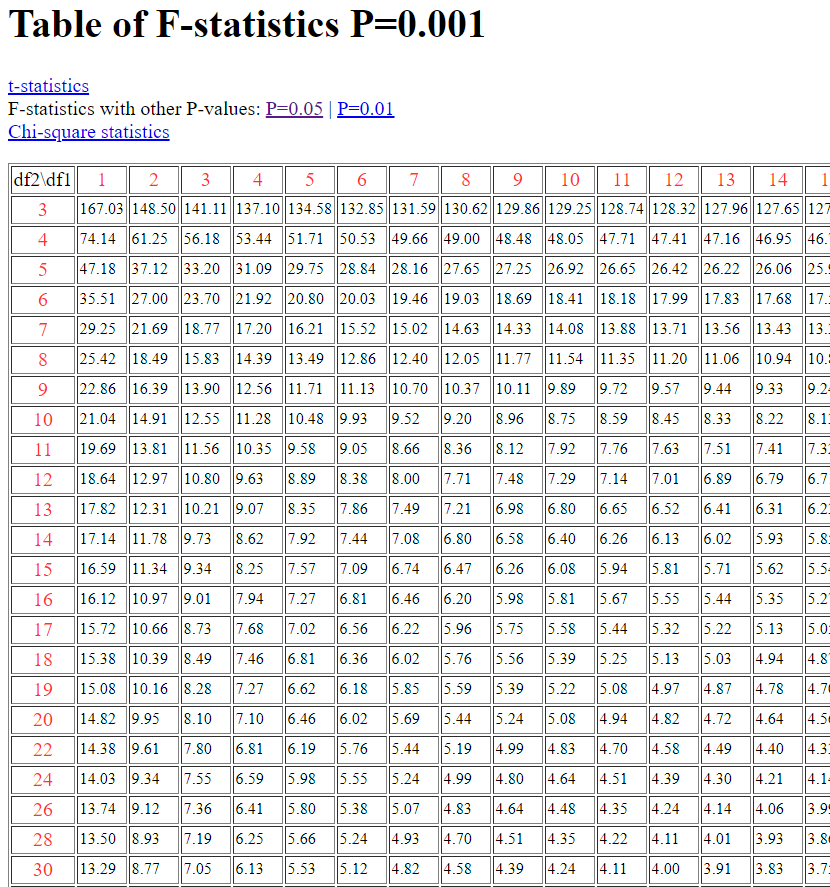
\includegraphics[width=0.3\linewidth]{ftable001} 

}

\caption{Tabla de Fisher p < 0.001}\label{fig:unnamed-chunk-9}
\end{figure}

Tabla tomada de
\url{https://web.ma.utexas.edu/users/davis/375/popecol/tables/f0001.html}

Para estos valores del \emph{F-Test}, al buscarlos en la tabla nos da
que el valor crítico es \(7.10\). Nuestro \emph{F-Test} da un resultado
de \(14.76\), que es mayor que el valor crítico, lo que significa que al
menos un tratamiento tiene un efecto medible sobre las observaciones y
es un resultado estadísticamente válido.

La explicación de lo anterior es:

ANOVA lo que hace es calcular varianzas. Estas varianzas nos indican
cuán alejados están los datos de la media, es decir, la dispersión de
los datos. Entre más grande sea la varianza, significa que los datos
están más lejos.

El \emph{F-test} lo que indica es la razón entre las varianzas de las
medias de la muestra y de las varianzas de los errores de las
observaciones de la muestra. La idea es que la varianza de las medias
debería de ser similar a la varianza de las observaciones en caso que
las diferencias de las observaciones sean por errores, dado que tienen
el mismo origen. De no ser así, la varianza de al menos un grupo de
medias sería mucho mayor que la varianza entre las muestras, porque
habría otro factor que está afectando solamente a ese grupo.

Tomando el ejemplo visto en clase, si partimos que cada observación se
compone de tres partes:

\[ y_{ij} = \mu + \tau_i + \epsilon_{ij} \]

\(\mu\) = la media \(\tau\) = Efecto del i-ésimo tratamiento
\(\epsilon\) = error de la observación

Tal y como vimos en clase, de esto podemos deducir dos hipótesis:

\begin{itemize}
\tightlist
\item
  Hipótesis nula \(H_0\): los efectos de los tratamientos no afectan, es
  decir, la media de todos los tratamientos es la misma, y todo puede
  ser explicado por \(\mu + \epsilon_{ij}\)
\item
  Hipótesis alternativa \(H_1\): Los efectos de los tratamientos si
  afectan, por lo tanto en al menos un par de tratamientos \((i,j)\),
  \(\mu_i \neq \mu_j\)
\end{itemize}

Para probar estas hipótesis, ANOVA lo que hace es calcular la dispersión
de las medias, y dividirlas por la dispersion de todas las
observaciones. Si \(\tau_i=0 \forall i\), entonces la dispersión de
todas las medias y la dispersión de todas las observaciones sería la
misma, y el \emph{F test} daría 1. De lo contrario daría un número mayor
que uno, al afectar \(\tau\) al menos a uno de los tratamientos moviendo
un poco la dispersión.

Adicionalmente, ANOVA utiliza los \emph{grados de libertad}. En el caso
de variables categóricas, como en este caso, para las medias se calcula
como uno menos que el numero de niveles \(DF_k=k-1\). En el caso del
error, se calcula como el número de observaciones menos el número de
niveles (o grupos) usados \(DF_n=n-k\).

El cálculo que realiza ANOVA es el siguiente:

\[
F=CMF
\]

\begin{itemize}
\tightlist
\item
  Lo llamado los \emph{mean squares}. Estos son
\end{itemize}

Esto se ve reflejado dentro de los datos en el objeto ANOVA:


\end{document}
